\documentclass{article}
    % General document formatting
    \usepackage[margin=0.7in]{geometry}
    \usepackage[parfill]{parskip}
    \usepackage[utf8]{inputenc}
    \usepackage{tikz}
    
    % Related to math
    \usepackage{amsmath,amssymb,amsfonts,amsthm}
    \usepackage{scrpage2}
	\pagestyle{scrheadings}
	
	% Kopfzeile
	\clearscrheadfoot
	\ihead{Tassilo Tanneberger}
	\chead{SRZ Aufgaben}
	\ohead{23.4.2020}
	
	\ofoot{\pagemark}
	
	\newcommand{\RN}[1]{%
  	\textup{\uppercase\expandafter{\romannumeral#1}}%
	}


\begin{document}

\section*{Wiederholung Sortier Algorithmen}

\subsection*{1.)}

\paragraph*{Iterativ - Bubble Sort}
basiert darauf das der aktuelle Wert immer mit dem Nächten Wert verglichen wird und dem entsprechend die beiden Werte getauscht (oder halt nicht) werden. Das muss n mal durchgeführt werden, um sicherzugehen das alles an der richtigen Position ist. Weil ja im Wort Case Szenario z.B die kleinste Zahl am Falschen ende, ist und somit n mal getauscht werden muss. Wobei n die Größe des zu sortierenden Datenfeldes ist.

\paragraph*{Recursiv - Quick Sort} 
basiert darauf das man ein Pivotelement setzt und alle Elemente die größer sind auf der einen Seite sammelt und die kleiner auf der anderen Seite des Pivotelements. Ist die größe der beiden Seiten größer 1. wird die Funktion wieder auf die beiden Seiten angewendet. So wird beim Rekursiven abstieg die Größe des sortierenden Felder immer kleiner bei einem neu rekursiven Neu-Aufruf der Funktion. Das Feld wird nicht direkt kleiner genauer gesagt schrinkt nur der betrachtete Abschnitt.

\subsection*{2.)}

Bubble Sort in der nicht optimierten Form hatt eine Komplexität von \( O(n ^ 2) \) im Vergleich dazu hatt Quick Sort im Average Case eine Komplexität von \( O( n \cdot log(n) ) \) was Quick-Sort den effizienteren Algorithmus macht. \newline

Die Komplexität eines Algorithmus gibt den mathematischen Zusammenhang zwischen Größe des Inputs und benötigter Operationen an z.B für Bubble Sort ist der Zusammenhang quadratisch. Das heißt, dass man immer eine Komplexität haben möchte, wo der Anstieg der benötigten Operationen nicht stark ansteigt.

\section*{Heap Sort}

\subsection*{2.)}

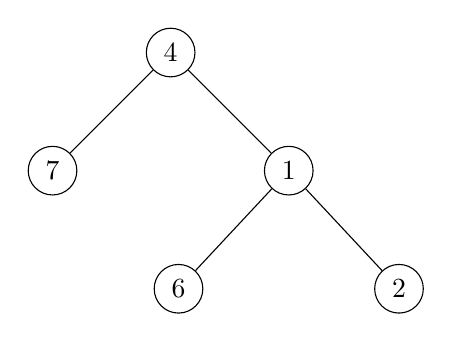
\begin{tikzpicture}[level distance=1.5cm,
  level 1/.style={sibling distance=3cm},
  level 2/.style={sibling distance=2.8cm},
  level 3/.style={sibling distance=1.5cm}]
\node[circle,draw](z){$ 4 $}
  child{
	node[circle,draw]{$ 7 $}  
  }
  child{
  node[circle,draw]{$ 1 $} 
  child{
   node[circle,draw] {$ 6 $}
  }
  child{   
  	node[circle,draw]{$ 2 $} 
  }
  };
\end{tikzpicture}


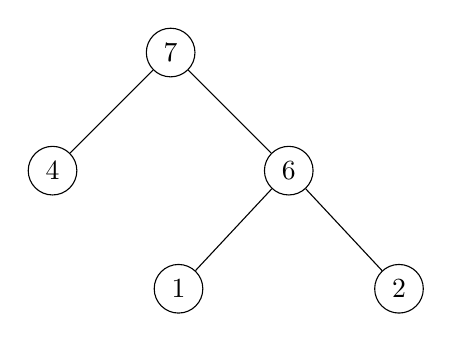
\begin{tikzpicture}[level distance=1.5cm,
  level 1/.style={sibling distance=3cm},
  level 2/.style={sibling distance=2.8cm},
  level 3/.style={sibling distance=1.5cm}]
\node[circle,draw](z){$ 7 $}
  child{
	node[circle,draw]{$ 4 $}  
  }
  child{
  node[circle,draw]{$ 6 $} 
  child{
   node[circle,draw] {$ 1 $}
  }
  child{   
  	node[circle,draw]{$ 2 $} 
  }
  };
\end{tikzpicture}

Sorted Array : [7]


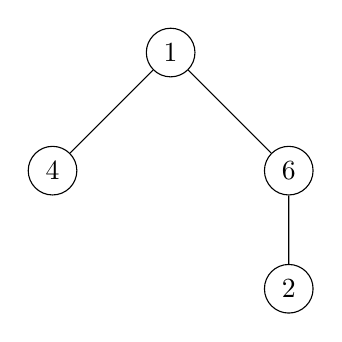
\begin{tikzpicture}[level distance=1.5cm,
  level 1/.style={sibling distance=3cm},
  level 2/.style={sibling distance=2.8cm},
  level 3/.style={sibling distance=1.5cm}]
\node[circle,draw](z){$ 1 $}
  child{
	node[circle,draw]{$ 4 $}  
  }
  child{
  node[circle,draw]{$ 6 $} 
  child{
   node[circle,draw] {$ 2 $}
  }
  };
\end{tikzpicture}

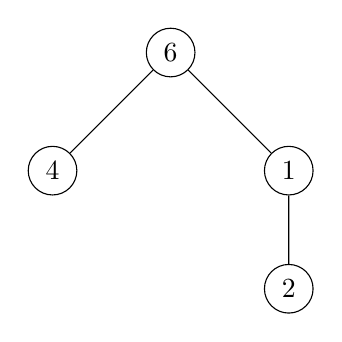
\begin{tikzpicture}[level distance=1.5cm,
  level 1/.style={sibling distance=3cm},
  level 2/.style={sibling distance=2.8cm},
  level 3/.style={sibling distance=1.5cm}]
\node[circle,draw](z){$ 6 $}
  child{
	node[circle,draw]{$ 4 $}  
  }
  child{
  node[circle,draw]{$ 1 $} 
  child{
   node[circle,draw] {$ 2 $}
  }
  };
\end{tikzpicture}

Sorted Array : [7,6]

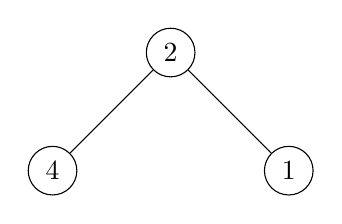
\begin{tikzpicture}[level distance=1.5cm,
  level 1/.style={sibling distance=3cm},
  level 2/.style={sibling distance=2.8cm},
  level 3/.style={sibling distance=1.5cm}]
\node[circle,draw](z){$ 2 $}
  child{
	node[circle,draw]{$ 4 $}  
  }
  child{
  node[circle,draw]{$ 1 $} 
  };
\end{tikzpicture}

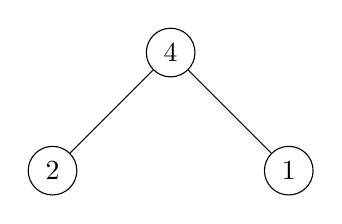
\begin{tikzpicture}[level distance=1.5cm,
  level 1/.style={sibling distance=3cm},
  level 2/.style={sibling distance=2.8cm},
  level 3/.style={sibling distance=1.5cm}]
\node[circle,draw](z){$ 4 $}
  child{
	node[circle,draw]{$ 2 $}  
  }
  child{
  node[circle,draw]{$ 1 $} 
  };
\end{tikzpicture}

Sorted Array : [7,6,4]

Und so weiter ...

\subsection*{3.)}

Zuerst muss der Binary Tree erstellt werden dafür werden die Werte aus dem Array in einen Binary Tree gefüllt.

Danach wird aus dem Binary Tree ein Max-Heap gemacht. Das passiert dadurch das man von den Blättern her anfängt und immer die Heapbedingung Ideal erfüllt (also im Falle des Max-Heap bedeutet, das Parent Node den größten Wert von den beiden Child Nodes und sich selber hatt). Wenn es zu einem Tausch kommt, muss logischerweise auch der Subbaum überprüft werden, ob die Heapbedingung noch überall erfüllt ist. Diese Methode wird meist "heapify" genannt.

Dann tauscht man den Wurzel Knoten mit dem tiefsten Blatt Knoten und zählt diesen nicht mehr zum Baum (Dieses Blatt fällt weg). Darauf folgend wird der Prozess wiederholt, bis nur noch ein Knoten des Baumes übrig ist.


\subsection*{4.)}

Da der Algorithmus ein in-place verfahren ist (er braucht keinen zusätzlichen Speicher) was ein Vorteil zu z.B MergeSort ist welche die gleiche Komplexität von \( O( n \cdot log(n) ) \) . Somit ist Heapsort z.B bei Embedded systems wo man nicht wirklich viel Speicher zur verfügung hatt besser geeignet. Oder einfach Datenfelder, die zu riesig sind und man nicht den nötigen extra Speicher hatt.

\end{document}




